\documentclass[letterpaper,12pt,fleqn]{article}
\usepackage{matharticle}
\usepackage{graphicx}
\usepackage{caption}
\pagestyle{empty}
\begin{document}
\section*{Lab 2: Syntax and Semantics}

At this point, it is important to make a distinction between \emph{syntax} and
\emph{semantics}. The numbers `$1$', `$2$', or `$1,000,000$' have no meaning in and of
themselves, just as the marks on a counting stick have no meaning outside of their
context. Likewise, the operations that we perform on numbers, like addition and
multiplication, have no intrinsic meaning until we connect them with some phenomenon in
nature that we are trying to model. We refer to the numbers and operations as
\emph{syntax}: the scribbles that we make on paper. The meaning that we attach to the
numbers and operations we call \emph{semantics}.

For a rather simple example, suppose that you have two piles of apples. One pile has
three apples and the other pile has two apples. In your mind (just like on a counting
stick) you associate the syntax '$3$' to represent the three apples in the first pile and
the syntax '$2$' to represent the two apples in the second pile. Then you realize that if
you combine the two piles, you will have $3+2=5$ apples. The syntax is, ``$3+2=5$'';
the semantics are, ``if you combine a pile of three apples with a pile of two apples
then you have a pile of five apples.''

This is how mathematics is used in the real world. We start with something in nature that
we wish to understand in order to explain what has happened (e.g., how fast was a car
traveling prior to impact in an accident) or to predict what will happen in the future
(e.g., how long will it take a rocket to travel to the space station and what course
should it take?). We then convert these semantics to mathematical syntax, usually in the
form of equations, and then use syntactic operations to find the answer that we want.
And then, lo and behold, the semantics of the syntactic answer will match reality! Just
like the apple example above. This is why mathematics is often called the language of the
universe.

\bigskip

\begin{figure}[h]
  \centering
  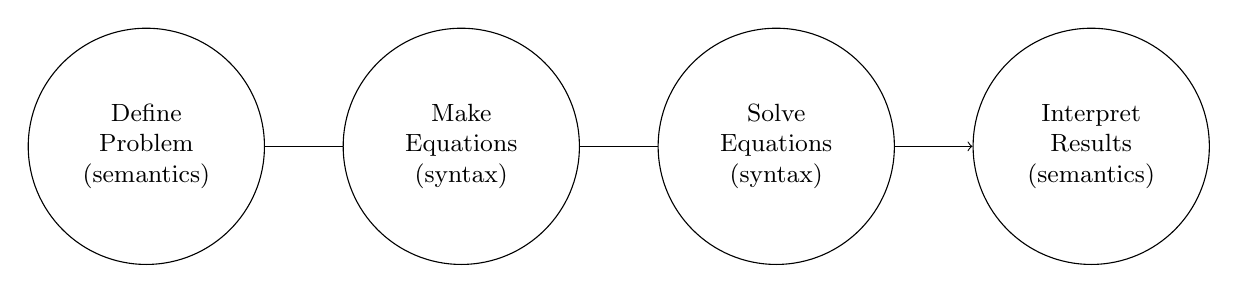
\begin{tikzpicture}
    \node [draw,circle,minimum size=3cm] (a) at (0,0)
          {\parbox{2cm}{\centering\small Define \\ Problem \\ (semantics)}};
    \node [draw,circle,minimum size=3cm] (b) at (4,0)
          {\parbox{2cm}{\centering\small Make \\ Equations \\ (syntax)}};
    \node [draw,circle,minimum size=3cm] (c) at (8,0)
          {\parbox{2cm}{\centering\small Solve \\ Equations \\ (syntax)}};
    \node [draw,circle,minimum size=3cm] (d) at (12,0)
          {\parbox{2cm}{\centering\small Interpret \\ Results \\ (semantics)}};
    \draw [->] (a) to (b) to (c) to (d);
  \end{tikzpicture}
  \caption*{Using Syntax and Semantics}
\end{figure}

\bigskip

In this course, we are going to focus a lot more on syntax than we are on semantics. This
can get frustrating because a lot of the examples and problems that we work on will seem
contrived and devoid of reality --- and this is true; however, you need to learn how to
use the tools before you can build a house. We will strive to introduce some real-world
semantics in the form of word problems whenever we can. You may have just groaned out
loud after reading that last sentence. Students seem to have a tremendous fear of word
problems. We are going to work hard to try and overcome that anxiety, because in the end,
it is the word problems that really count; the syntax is just a means of getting to an
answer.

\subsection*{Questions}

\begin{enumerate}
\item Identify which of the following represents syntax and which represents semantics.
  Don't worry about the complexity of the problem. Many times, when we approach a
  problem, we need to initially ignore the complexity until we can identify what is
  going on at a higher level:
  \begin{enumerate}
  \item The kinetic energy of a moving object is directly proportional to the mass
    of the object and the square of its velocity.

    \vspace{0.5in}
    
  \item $K=\frac{1}{2}mv^2$

    \vspace{0.5in}
  \end{enumerate}

\item You work for a construction company. Your boss wants to move four piles of
  bricks, each pile weighing $500$ pounds, to a construction site. The company truck can
  carry a maximum load of $2,500$ pounds. Your boss asks you if he can transport the
  entire load of bricks in one trip.
  \begin{enumerate}
  \item Using mathematical syntax, express how you would calculate the total weight
    of the four piles of bricks. Your syntax should include the weight of each pile, the
    number of piles, a mathematical operation, and an answer, all in the form of an
    equation.

    \vspace{1in}
    
  \item Interpret your syntactic answer in order to answer your boss's question.
  \end{enumerate}
\end{enumerate}

\end{document}
